\section{Results}\label{sec:results}

Every result in this section is pre-registered unless marked as a re-report or as descriptive. Scores are means of the \code{kleos\_policy} grader on the 349-item benchmark. Intervals are 95\% bootstrap intervals, item-level for the H1 comparisons and cluster-level by perturbation group from H8 on, as the protocol fixes. Table~\ref{tab:main} collects the main numbers, Table~\ref{tab:per-task} the per-task results, Table~\ref{tab:head-to-head} the comparisons between fine-tuned models and Table~\ref{tab:subscores} the grader sub-scores; Figures~\ref{fig:main} to \ref{fig:forest} draw them.

% Figure 3: mean kleos_policy score on the 349-item benchmark, base + orchestration (arm1)
% vs fine-tuned (arm2), with the recorded example-level 95% bootstrap intervals.
% source: pilot, docs/experiments.md H1 corrected scores (EXP:167): 0.4744 / 0.8015; no corrected
%   interval is recorded for the baseline, so neither pilot bar carries one.
% source: Hermes report (HER:259-262): arm1 0.4755 [0.4532-0.4978], arm2 0.8051 [0.7813-0.8288].
% source: Logos v0.0.1 report (L1:291-294): arm1 0.4469 [0.4219-0.4720], arm2 0.7896 [0.7644-0.8147].
% source: Logos v0.0.2, docs/experiments.md H9 result (EXP:790-791): arm2 0.8596, descriptive, no arm1.
% The error-bar lengths are the distances from each mean to its recorded interval endpoints.
\begin{figure}[t]
\centering
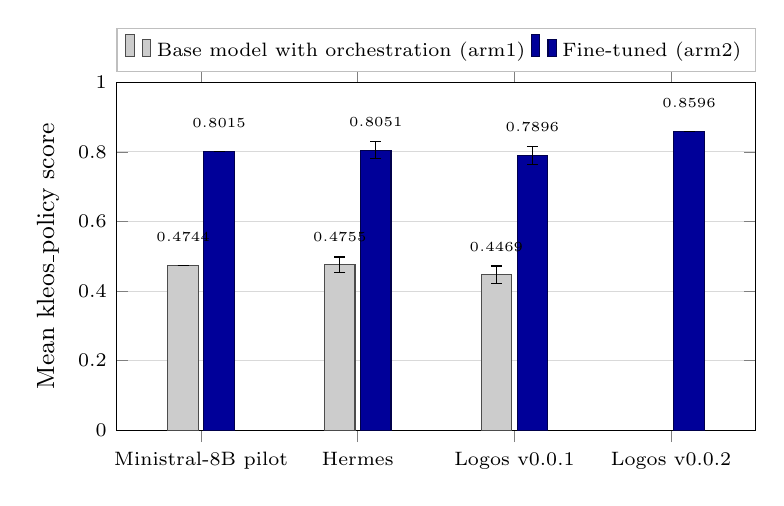
\begin{tikzpicture}
\begin{axis}[
  ybar, bar width=11pt,
  width=0.8\linewidth, height=6cm,
  ylabel={Mean \code{kleos\_policy} score}, ymin=0, ymax=1.0,
  symbolic x coords={Ministral-8B pilot, Hermes, Logos v0.0.1, Logos v0.0.2},
  xtick={Ministral-8B pilot, Hermes, Logos v0.0.1, Logos v0.0.2}, enlarge x limits=0.18,
  ytick={0,0.2,0.4,0.6,0.8,1.0},
  ymajorgrids, grid style={gray!30},
  legend style={at={(0.5,1.03)}, anchor=south, legend columns=2, font=\scriptsize, draw=gray!50}, legend cell align=left,
  tick label style={font=\scriptsize}, label style={font=\small},
  nodes near coords, nodes near coords style={font=\tiny, yshift=5pt, /pgf/number format/.cd, fixed, precision=4},
  error bars/y dir=both, error bars/y explicit,
  error bars/error bar style={black, thin},
]
\addplot[fill=gray!40, draw=gray!60!black] plot[error bars/.cd, y dir=both, y explicit] table[x=model, y=score, y error plus=ep, y error minus=em] {
model score ep em
{Ministral-8B pilot} 0.4744 0 0
{Hermes} 0.4755 0.0223 0.0223
{Logos v0.0.1} 0.4469 0.0251 0.0250
};
\addlegendentry{Base model with orchestration (arm1)}
\addplot[fill=blue!60!black, draw=blue!30!black] plot[error bars/.cd, y dir=both, y explicit] table[x=model, y=score, y error plus=ep, y error minus=em] {
model score ep em
{Ministral-8B pilot} 0.8015 0 0
{Hermes} 0.8051 0.0237 0.0238
{Logos v0.0.1} 0.7896 0.0251 0.0252
{Logos v0.0.2} 0.8596 0 0
};
\addlegendentry{Fine-tuned (arm2)}
\end{axis}
\end{tikzpicture}
\caption{Mean \code{kleos\_policy} score on the 349-item benchmark. Error bars are the recorded item-level 95\% bootstrap intervals (Hermes and Logos v0.0.1 only; the pilot baseline was re-graded after its interval was recorded, and the Logos v0.0.2 overall mean is descriptive). Logos v0.0.2 has no base arm. Item-level intervals treat the 349 items as independent and are narrower than the cluster intervals used from H8 on (Section~\ref{sec:protocol}).}
\label{fig:main}
\end{figure}

% Figure 4: per-task gain (arm2 - arm1) for the three runs with a base arm.
% source: pilot, docs/experiments.md H1 corrected table (EXP:157-165).
% source: Hermes report per-task table (HER:266-275).
% source: Logos v0.0.1, docs/experiments.md H8a table (EXP:594-603).
% Task order is the data-contract order; n is the test count per task.
\begin{figure}[t]
\centering
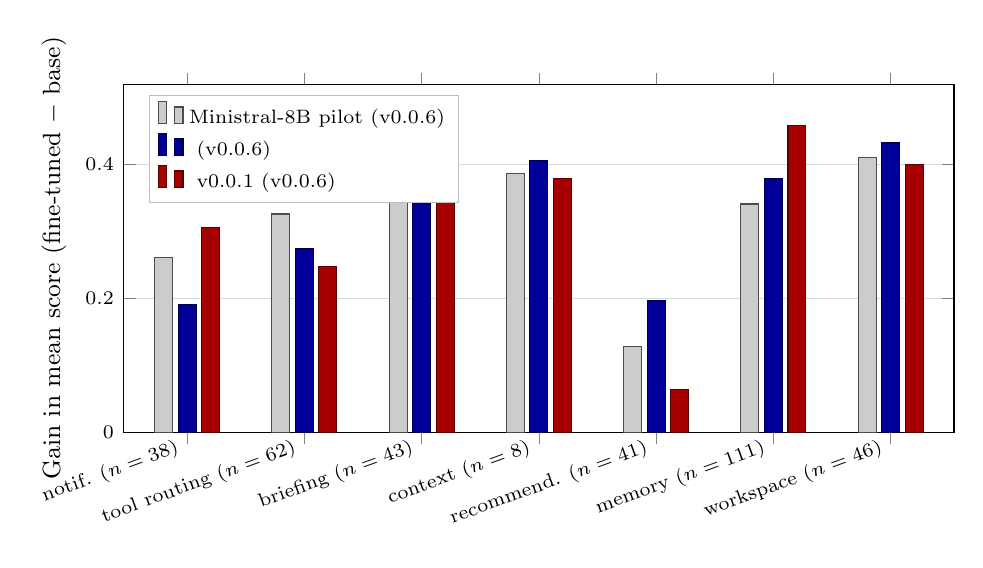
\begin{tikzpicture}
\begin{axis}[
  ybar, bar width=6.5pt,
  width=\linewidth, height=6cm,
  ylabel={Gain in mean score (fine-tuned $-$ base)}, ymin=0, ymax=0.52,
  symbolic x coords={notif. ($n=38$), tool routing ($n=62$), briefing ($n=43$), context ($n=8$), recommend. ($n=41$), memory ($n=111$), workspace ($n=46$)},
  xtick=data, x tick label style={font=\scriptsize, rotate=20, anchor=east},
  enlarge x limits=0.09,
  ymajorgrids, grid style={gray!30},
  legend pos=north west, legend cell align=left, legend style={font=\scriptsize, draw=gray!50},
  tick label style={font=\scriptsize}, label style={font=\small},
]
\addplot[fill=gray!40, draw=gray!60!black] coordinates {
  (notif. ($n=38$),0.2617) (tool routing ($n=62$),0.3262) (briefing ($n=43$),0.4385) (context ($n=8$),0.3870)
  (recommend. ($n=41$),0.1284) (memory ($n=111$),0.3412) (workspace ($n=46$),0.4108)};
\addlegendentry{Ministral-8B pilot (v0.0.6)}
\addplot[fill=blue!60!black, draw=blue!30!black] coordinates {
  (notif. ($n=38$),0.1904) (tool routing ($n=62$),0.2750) (briefing ($n=43$),0.4035) (context ($n=8$),0.4065)
  (recommend. ($n=41$),0.1971) (memory ($n=111$),0.3798) (workspace ($n=46$),0.4323)};
\addlegendentry{\hermes{} (v0.0.6)}
\addplot[fill=red!65!black, draw=red!35!black] coordinates {
  (notif. ($n=38$),0.3054) (tool routing ($n=62$),0.2479) (briefing ($n=43$),0.4094) (context ($n=8$),0.3792)
  (recommend. ($n=41$),0.0643) (memory ($n=111$),0.4586) (workspace ($n=46$),0.4005)};
\addlegendentry{\logos{} v0.0.1 (v0.0.6)}
\end{axis}
\end{tikzpicture}
\caption{Per-task gain from fine-tuning on the 349-item benchmark, by task (test items per task in parentheses). Every pilot and Hermes gain was significant under the pre-registered item-level bootstrap ($p<0.05$ and $p<0.001$ respectively); for Logos v0.0.1, five tasks improved under the cluster bootstrap, \code{recommendation\_generation} did not reach significance, and \code{context\_prioritization} (8 items, fewer than 5 groups) was not estimable by groups. Per-task intervals are not recorded, so no error bars are drawn (Table~\ref{tab:per-task}).}
\label{fig:tasks}
\end{figure}

% Figure 5: the six recorded paired cluster-bootstrap differences between fine-tuned models.
% source: H8b primary and should-decline rows, docs/experiments.md (EXP:545-549, 564):
%   answerable -0.0168 [-0.0546, +0.0177]; should-decline -0.0111 [-0.0429, +0.0195].
% source: H9 primary row (EXP:748-752) and should-decline row (EXP:768-770; L2:166):
%   answerable +0.0409 [+0.0040, +0.0780]; should-decline +0.1020 [-0.0018, +0.2062].
% source: Logos v0.0.1 -> v0.0.2, Logos v0.0.2 report section 8 (L2:204-210):
%   answerable +0.0577 [+0.0234, +0.0952]; should-decline +0.1131 [+0.0028, +0.2296].
% Answerable rows resample 61 groups, should-decline rows 17. Error-bar lengths are the
% distances from each estimate to its recorded interval endpoints.
\begin{figure}[t]
\centering
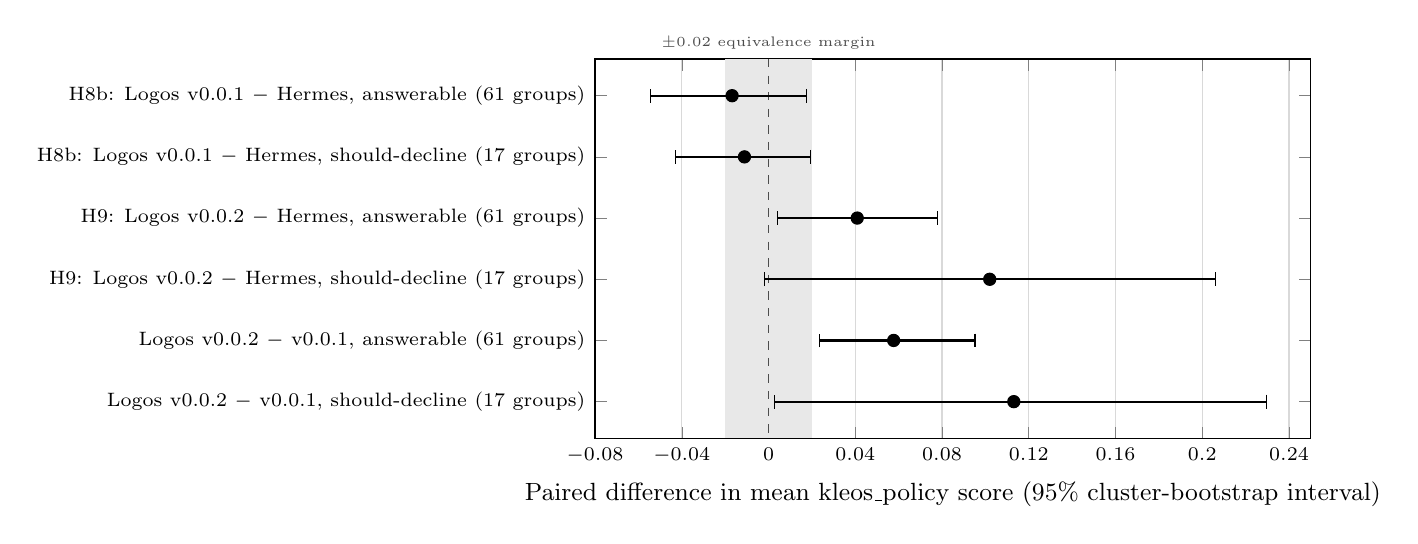
\begin{tikzpicture}
\begin{axis}[
  width=0.88\linewidth, height=6.4cm,
  xlabel={Paired difference in mean \code{kleos\_policy} score (95\% cluster-bootstrap interval)},
  xmin=-0.08, xmax=0.25,
  xtick={-0.08,-0.04,0,0.04,0.08,0.12,0.16,0.20,0.24},
  scaled x ticks=false, xticklabel style={/pgf/number format/fixed, /pgf/number format/precision=2},
  ymin=0.4, ymax=6.6, y dir=reverse,
  ytick={1,2,3,4,5,6},
  yticklabels={
    {H8b: Logos v0.0.1 $-$ Hermes, answerable (61 groups)},
    {H8b: Logos v0.0.1 $-$ Hermes, should-decline (17 groups)},
    {H9: Logos v0.0.2 $-$ Hermes, answerable (61 groups)},
    {H9: Logos v0.0.2 $-$ Hermes, should-decline (17 groups)},
    {Logos v0.0.2 $-$ v0.0.1, answerable (61 groups)},
    {Logos v0.0.2 $-$ v0.0.1, should-decline (17 groups)}},
  y tick label style={font=\scriptsize, align=right},
  tick label style={font=\scriptsize}, label style={font=\small},
  xmajorgrids, grid style={gray!30},
  clip=false,
]
\fill[gray!18] (axis cs:-0.02,0.4) rectangle (axis cs:0.02,6.6);
\draw[dashed, gray!60!black] (axis cs:0,0.4) -- (axis cs:0,6.6);
\node[font=\tiny, gray!60!black, anchor=south] at (axis cs:0,0.4) {$\pm 0.02$ equivalence margin};
\addplot[only marks, mark=*, mark size=2.2pt, color=black,
  error bars/.cd, x dir=both, x explicit, error bar style={thick}, error mark options={rotate=90, mark size=2.5pt}]
  table[x=est, y=row, x error plus=ep, x error minus=em] {
est row ep em
-0.0168 1 0.0345 0.0378
-0.0111 2 0.0306 0.0318
0.0409 3 0.0371 0.0369
0.1020 4 0.1042 0.1038
0.0577 5 0.0375 0.0343
0.1131 6 0.1165 0.1103
};
\end{axis}
\end{tikzpicture}
\caption{Paired differences between fine-tuned models, resampled by benchmark group (2,000 resamples). The primary rows are the answerable ones: H8b is inconclusive because its interval crosses zero and is not contained in the $\pm 0.02$ equivalence margin, and H9 is ``better'' because its interval lies entirely above zero. The should-decline rows rest on 17 groups; only the v0.0.1 to v0.0.2 row excludes zero.}
\label{fig:forest}
\end{figure}


% source: pilot EXP:167, 182-198; Hermes HER:259-262, HMD:110-111, L1:416-418, HMD:135-136; Logos v0.0.1 L1:291-294, EXP:605-613; Logos v0.0.2 EXP:748-752, 787-791, L2:154-176.
\begin{table}[t]
\centering\scriptsize
\caption{Main results on the 349-item benchmark. Base and fine-tuned intervals are item-level; the answerable and should-decline columns are re-reports by group with cluster intervals where recorded. The pilot's baseline was re-graded after its interval was recorded, so neither pilot figure carries one; Logos v0.0.2 has no base arm and its overall mean is descriptive. Consistency is the agreement rate by perturbation group, where a perfect model scores 1.000. Sources: \code{docs/experiments.md} (H1, H8, H9 entries) and the run reports.}
\label{tab:main}
\begin{tabular}{L{19mm}L{21mm}L{21mm}L{26mm}L{27mm}L{20mm}L{16mm}}
\toprule
Model & Base, arm1 & Fine-tuned, arm2 & Difference & Answerable (271 items, 61 groups), arm2 & Should-decline (78 items, 17 groups), arm2 & Consistency, arm2 (all / answerable) \\
\midrule
Ministral-8B pilot & 0.4744 & 0.8015 & $+0.3271$; 7 of 7 tasks $p<0.05$ & not reported & not reported & not reported \\
\hermes{} & 0.4755 \ci{0.4532}{0.4978} & 0.8051 \ci{0.7813}{0.8288} & $+0.3295$ \ci{0.3068}{0.3521}, $p<0.001$ & 0.8976 \ci{0.8634}{0.9301} (base 0.5570) & 0.4835 (base 0.1923) & 0.769 / 0.770 (base 0.346) \\
\logos{} v0.0.1 & 0.4469 \ci{0.4219}{0.4720} & 0.7896 \ci{0.7644}{0.8147} & $+0.3427$ (descriptive); answerable $+0.3952$ \ci{+0.3443}{+0.4438} & 0.8808 \ci{0.8381}{0.9191} (base 0.4857 \ci{0.4445}{0.5261}) & 0.4724 (base 0.3123; $+0.1601$ \ci{+0.0712}{+0.2409}) & 0.833 / 0.853 (base 0.154 / 0.164) \\
\logos{} v0.0.2 & not run & 0.8596 (descriptive) & --- & 0.9385 \ci{0.9083}{0.9663} & 0.5855 & 0.833 / 0.869 \\
\bottomrule
\end{tabular}
\end{table}

\subsection{H1: the pilot and its replication}
% source: EXP:157-198 (pilot per task, F1 re-grade); HER:259-320 (Hermes arms, per task, sub-scores); HER:384-437 and EXP:103-108 (descriptive comparison); HMD:110-111, L1:416-418, HMD:135-136 (subsets and consistency by group).
The pilot run on Ministral-8B compared the orchestrated base against the fine-tuned adapter on all 349 items. Its first report scored the baseline at 0.5231. An artifact audit then found that nDCG could exceed 1.0 on a ranking that repeats an item (finding F1), and 60\% of the baseline's answers repeated one. Bounding nDCG re-graded 210 of the 349 baseline responses and none of the fine-tuned ones, moved the baseline to 0.4744, left the fine-tuned score at 0.8015, and raised the count of tasks with a significant improvement from six to seven. The corrected gap is $+0.3271$, with every task improved at $p<0.05$ under the pre-registered item-level bootstrap (Table~\ref{tab:per-task}, first block); parse failures fell from 13 to 0 (descriptive).

\hermes{} replicated the result on a different base one week later: 0.4755 \ci{0.4532}{0.4978} to 0.8051 \ci{0.7813}{0.8288}, a paired difference of $+0.3295$ \ci{0.3068}{0.3521}. The comparison tool prints $p = 0.0$, meaning that none of the 2,000 resamples crossed zero, so the correct statement is $p<0.001$. Every task improved with $p<0.001$ (Table~\ref{tab:per-task}, second block; Figure~\ref{fig:tasks}), from $+0.1904$ on notification prioritization to $+0.4323$ on workspace reasoning; the 8-item context-prioritization task moved from 0.5935 to 1.0000 (interval 0.2612 to 0.5352). The sub-scores (Table~\ref{tab:subscores}) show where the gain comes from: the ranking component rose from 0.5985 to 0.8822 (nDCG 0.6174 to 0.9527, top-1 accuracy 0.5702 to 0.7765, Kendall's $\tau$ 0.5449 to 0.8479), the deciding factor from 0.0860 to 0.6132 and confidence from 0.7421 to 0.9198. \code{format\_valid} is 0.0000 in both arms with 0 parse failures: neither arm produced the held-out JSON format, and the scores measure judgment on prose answers. Descriptively, fine-tuning also shortened the answers, from a mean of 226 completion tokens to 94 (medians 217 and 91); one baseline answer hit the 512-token cap and no fine-tuned answer did; mean latency on the T4 fell from 24.7\,s to 16.1\,s. Re-reported by group after the H8 amendment, Hermes scores 0.8976 \ci{0.8634}{0.9301} on the 271 answerable items (base 0.5570) and 0.4835 on the 78 should-decline items (base 0.1923), and its agreement rate by group is 0.769 (base 0.346).

The two fine-tuned models land within 0.004 of each other overall (0.8015 and 0.8051) and the two baselines within 0.002; the per-task differences between the adapters range from $-0.0766$ on notification prioritization to $+0.1076$ on context prioritization. The record treats these as leads, not results: scale, architecture and pretraining are confounded between the two bases, and the agreement is cross-base consistency, not a replication of one configuration across seeds.

% source: pilot EXP:157-165; Hermes HER:266-275; Logos v0.0.1 EXP:594-603.
\begin{table}[t]
\centering\scriptsize
\caption{Per-task results for the three runs with a base arm. Verdicts for the pilot and Hermes are under the pre-registered item-level bootstrap; verdicts for Logos v0.0.1 are under the cluster bootstrap by group (the item-level verdict is given where it differs). Per-task intervals are not recorded except the one shown. Sources: \code{docs/experiments.md} H1 and H8a tables; Hermes run report.}
\label{tab:per-task}
\begin{tabular}{L{40mm}R{8mm}R{14mm}R{16mm}R{14mm}L{54mm}}
\toprule
Task & $n$ & Base & Fine-tuned & Difference & Verdict \\
\midrule
\multicolumn{6}{l}{\emph{Ministral-8B pilot, corrected after F1 (2026-09-15)}} \\
mission-control briefing & 43 & 0.5323 & 0.9708 & $+0.4385$ & improved, $p<0.05$ \\
workspace reasoning & 46 & 0.5228 & 0.9336 & $+0.4108$ & improved, $p<0.05$ \\
context prioritization & 8 & 0.5054 & 0.8924 & $+0.3870$ & improved, $p<0.05$ \\
memory-conflict resolution & 111 & 0.4781 & 0.8192 & $+0.3412$ & improved, $p<0.05$ \\
tool routing & 62 & 0.3919 & 0.7181 & $+0.3262$ & improved, $p<0.05$ \\
notification prioritization & 38 & 0.6253 & 0.8871 & $+0.2617$ & improved, $p<0.05$ \\
recommendation generation & 41 & 0.3285 & 0.4569 & $+0.1284$ & improved, $p<0.05$ \\
overall & 349 & 0.4744 & 0.8015 & $+0.3271$ & 7 of 7 tasks improved \\
\midrule
\multicolumn{6}{l}{\emph{\hermes{} (2026-09-22)}} \\
workspace reasoning & 46 & 0.5190 & 0.9512 & $+0.4323$ & improved, $p<0.001$ \\
context prioritization & 8 & 0.5935 & 1.0000 & $+0.4065$ & improved, $p<0.001$; interval 0.2612 to 0.5352 \\
mission-control briefing & 43 & 0.5681 & 0.9716 & $+0.4035$ & improved, $p<0.001$ \\
memory-conflict resolution & 111 & 0.4756 & 0.8553 & $+0.3798$ & improved, $p<0.001$ \\
tool routing & 62 & 0.3929 & 0.6679 & $+0.2750$ & improved, $p<0.001$ \\
recommendation generation & 41 & 0.2974 & 0.4946 & $+0.1971$ & improved, $p<0.001$ \\
notification prioritization & 38 & 0.6201 & 0.8105 & $+0.1904$ & improved, $p<0.001$ \\
overall & 349 & 0.4755 & 0.8051 & $+0.3295$ & interval 0.3068 to 0.3521, $p<0.001$ \\
\midrule
\multicolumn{6}{l}{\emph{\logos{} v0.0.1, H8a (2026-10-01), verdicts by group}} \\
memory-conflict resolution & 111 & 0.3763 & 0.8350 & $+0.4586$ & improved, $p<0.001$ \\
mission-control briefing & 43 & 0.5552 & 0.9646 & $+0.4094$ & improved, $p<0.001$ \\
workspace reasoning & 46 & 0.5366 & 0.9370 & $+0.4005$ & improved, $p<0.001$ \\
context prioritization & 8 & 0.6204 & 0.9995 & $+0.3792$ & not estimable by group (8 items); improved by item, $p<0.001$ \\
notification prioritization & 38 & 0.5888 & 0.8942 & $+0.3054$ & improved, $p<0.001$ \\
tool routing & 62 & 0.4021 & 0.6501 & $+0.2479$ & improved, $p<0.001$ \\
recommendation generation & 41 & 0.3263 & 0.3906 & $+0.0643$ & not significant \\
overall & 349 & 0.4469 & 0.7896 & $+0.3427$ & descriptive; 5 tasks improved, none regressed: supported \\
\bottomrule
\end{tabular}
\end{table}

\subsection{H8: a stronger base}
% source: H8a EXP:594-613, L1:291-300, 321-327; H8b EXP:545-576, L1:395-437.
\paragraph{H8a (supported).} Fine-tuning helped the Ministral 3 base as it had helped the others: Logos v0.0.1 moved from 0.4469 \ci{0.4219}{0.4720} to 0.7896 \ci{0.7644}{0.8147} overall. Under the cluster bootstrap five tasks improved with $p<0.001$ and none regressed (Table~\ref{tab:per-task}, third block); recommendation generation ($+0.0643$) was not significant, and the 8-item context-prioritization task was not estimable by group. On the answerable subset the paired cluster difference is $+0.3952$ \ci{+0.3443}{+0.4438} (0.4857 to 0.8808) and on the should-decline subset $+0.1601$ \ci{+0.0712}{+0.2409} (0.3123 to 0.4724); agreement by group rose from 0.154 to 0.833. One caveat is recorded beside these gains: 41 of the base's 349 answers (11.7\%) were cut at the 512-token budget, against none of the adapter's (mean completion length 348 against 95 tokens), which may inflate the base-to-adapter differences.

\paragraph{H8b (inconclusive).} On the primary population Hermes scores 0.8976 \ci{0.8634}{0.9301} and Logos v0.0.1 0.8808 \ci{0.8381}{0.9191}; the paired cluster difference over 61 groups is $-0.0168$ \ci{-0.0546}{+0.0177} (Table~\ref{tab:head-to-head}, Figure~\ref{fig:forest}). The interval crosses zero and is not contained in the $\pm 0.02$ equivalence margin, so the pre-registered verdict is inconclusive: a Hermes lead of up to 0.0546 is not ruled out, nor is a Logos lead of up to 0.0177. The secondary rows point the same way. On the should-decline subset the difference is $-0.0111$ \ci{-0.0429}{+0.0195}. Per task, recommendation generation regressed from 0.4946 to 0.3906 ($-0.1040$; $p = 0.006$ by group, $p<0.001$ by item) and workspace reasoning by $-0.0142$ ($p = 0.014$ by group, not significant by item); notification prioritization rose by $+0.0837$ ($p = 0.007$ by item, not significant by group); the other three estimable tasks' group intervals included zero (per-task intervals are not recorded). Agreement by group was higher for Logos (0.833 against 0.769; 0.853 against 0.770 on answerable groups), with no interval computed (descriptive). The overall means, 0.8051 and 0.7896, are descriptive.

\subsection{H9: a Logos trained to think}
% source: EXP:748-791; L2:136-145, 154-176, 185-194, 204-210.
\paragraph{H9 (supported: better).} Logos v0.0.2 scores 0.9385 \ci{0.9083}{0.9663} on the answerable items against Hermes' 0.8976 \ci{0.8634}{0.9301}; the paired cluster difference over 61 groups is $+0.0409$ \ci{+0.0040}{+0.0780}, $p = 0.031$. The interval lies entirely above zero, so the pre-registered verdict is better; the record notes that the lower bound is close to zero. The first secondary row, the one the v0.0.7 data was built to move, did not reach significance by group: on the should-decline items Logos v0.0.2 scores 0.5855 against 0.4835, $+0.1020$ \ci{-0.0018}{+0.2062}, $p = 0.054$ over 17 groups. By task, notification prioritization ($+0.1324$, $p<0.001$), recommendation generation ($+0.0893$, $p = 0.002$) and memory-conflict resolution ($+0.0737$, $p = 0.048$) improved; tool routing ($+0.0330$), workspace reasoning ($+0.0172$) and mission-control briefing ($-0.0153$) had group intervals that included zero; context prioritization ($-0.0002$) was not estimable. Descriptively, agreement by group rose from 0.769 to 0.833 over all groups and from 0.770 to 0.869 over the answerable ones. The overall mean, 0.8596, is descriptive: v0.0.2 has no base arm.

\paragraph{Logos v0.0.1 to v0.0.2 (secondary).} Against its own predecessor, v0.0.2 gains $+0.0577$ \ci{+0.0234}{+0.0952} on the answerable items ($p<0.001$) and $+0.1131$ \ci{+0.0028}{+0.2296} on the should-decline items ($p = 0.046$); recommendation generation ($+0.1933$, $p<0.001$) and memory-conflict resolution ($+0.0941$, $p = 0.005$) improved and no task regressed. Among the comparisons between fine-tuned models, this is the one in which the should-decline difference excludes zero, and it confounds the same three changes as H9.

\paragraph{The traces (descriptive).} All 349 v0.0.2 completions carried a reasoning trace and every trace closed; the traces average 549 characters (median 540, maximum 840) against 575 in the validation targets. Completions averaged 293.5 tokens (median 285, 95th percentile 413) and took 53.8\,s on average on the two T4s (95th percentile 76.3\,s). Six completions reached the 1,024-token budget after a closed trace, all on answerable memory-conflict items, where the answer repeated a phrase; they were scored as generated, at 0.59 to 0.65 each. \code{format\_valid} is 0.0 for all three models.

\par\medskip\noindent\fbox{\parbox{\dimexpr\linewidth-2\fboxsep-2\fboxrule\relax}{\small\textbf{Reported, not decisive.} The secondary rows in this section are uncorrected for multiple comparisons. Three sit near the conventional threshold: memory-conflict resolution under H9 ($p = 0.048$ by group), the H9 should-decline row ($p = 0.054$) and the v0.0.1 to v0.0.2 should-decline row ($p = 0.046$). None of them bears on the pre-registered verdicts, which rest on the primary rows alone.}}

% source: H8b EXP:545-576, L1:429-437; H9 EXP:748-791, L2:165-176; v0.0.1 to v0.0.2 L2:204-210.
\begin{table}[t]
\centering\scriptsize
\caption{Comparisons between fine-tuned models. Every interval is a paired cluster-bootstrap 95\% interval by group; per-task rows give the difference and the verdict by group, with the item-level verdict where it differs. Consistency is the agreement rate by group. Per-task intervals are not recorded; ``n.s.'' is the recorded verdict that the group interval included zero. Sources: \code{docs/experiments.md} H8b and H9 results; Logos v0.0.1 and v0.0.2 run reports.}
\label{tab:head-to-head}
\begin{tabular}{L{27mm}L{40mm}L{40mm}L{40mm}}
\toprule
Row & H8b: Logos v0.0.1 $-$ Hermes & H9: Logos v0.0.2 $-$ Hermes & Logos v0.0.2 $-$ v0.0.1 (secondary) \\
\midrule
Answerable, 271 items, 61 groups (primary) & $-0.0168$ \ci{-0.0546}{+0.0177}; inconclusive & $+0.0409$ \ci{+0.0040}{+0.0780}, $p = 0.031$; better & $+0.0577$ \ci{+0.0234}{+0.0952}, $p<0.001$ \\
Should-decline, 78 items, 17 groups & $-0.0111$ \ci{-0.0429}{+0.0195} & $+0.1020$ \ci{-0.0018}{+0.2062}, $p = 0.054$; not significant & $+0.1131$ \ci{+0.0028}{+0.2296}, $p = 0.046$ \\
Per task, by group & recommendation $-0.1040$ regressed ($p = 0.006$); workspace $-0.0142$ regressed ($p = 0.014$; n.s.\ by item); notification $+0.0837$ n.s.\ (improved by item, $p = 0.007$); briefing $-0.0070$, tool routing $-0.0178$, memory $-0.0204$ n.s.; context not estimable & notification $+0.1324$ ($p<0.001$), recommendation $+0.0893$ ($p = 0.002$), memory $+0.0737$ ($p = 0.048$) improved; tool routing $+0.0330$, workspace $+0.0172$, briefing $-0.0153$ n.s.; context $-0.0002$ not estimable & recommendation $+0.1933$ ($p<0.001$), memory $+0.0941$ ($p = 0.005$) improved; no task regressed \\
Consistency by group, all / answerable & 0.769 / 0.770 $\rightarrow$ 0.833 / 0.853 & 0.769 / 0.770 $\rightarrow$ 0.833 / 0.869 & 0.833 / 0.853 $\rightarrow$ 0.833 / 0.869 \\
Overall mean (descriptive) & 0.8051 vs 0.7896 & 0.8051 vs 0.8596 & 0.7896 vs 0.8596 \\
\bottomrule
\end{tabular}
\end{table}

% source: Hermes HER:310-320; Logos v0.0.1 L1:343-352.
\begin{table}[t]
\centering\small
\caption{Grader sub-scores on the full benchmark. The score is the mean of the ranking, deciding-factor and confidence components where the reference supports them; \code{format\_valid} is reported and excluded. Sources: Hermes and Logos v0.0.1 run reports.}
\label{tab:subscores}
\begin{tabular}{lrrrr}
\toprule
Sub-score & Hermes base & Hermes fine-tuned & Logos v0.0.1 base & Logos v0.0.1 fine-tuned \\
\midrule
score (\code{judgment}) & 0.4755 & 0.8051 & 0.4469 & 0.7896 \\
ranking & 0.5985 & 0.8822 & 0.4468 & 0.8529 \\
\quad nDCG & 0.6174 & 0.9527 & 0.4505 & 0.9459 \\
\quad top-1 accuracy & 0.5702 & 0.7765 & 0.4413 & 0.7135 \\
\quad Kendall's $\tau$ & 0.5449 & 0.8479 & 0.5350 & 0.8345 \\
deciding factor & 0.0860 & 0.6132 & 0.1805 & 0.5989 \\
confidence & 0.7421 & 0.9198 & 0.7135 & 0.9169 \\
\code{format\_valid} & 0.0000 & 0.0000 & 0.0000 & 0.0000 \\
parse failures & 0 & 0 & 0 & 0 \\
\bottomrule
\end{tabular}
\end{table}
